% !TEX root = obbvi-uai.tex
\section{EMPIRICAL STUDY}
\label{sec:experiments}
\glsresetall{}

We study our method with two non-conjugate probabilistic models: the
\gls{GNTS} and the Poisson \gls{DEF}. We found that \gls{OBBVI}
reduces the variance of the \gls{BBVI} estimator and leads to faster
convergence.

\vspace*{-5pt}
\subsection{Description of the experiments}
\label{sec:descr_experiments}
\vspace*{-5pt}

\parhead{Models description and datasets.}
The \gls{GNTS} model \citep{Ranganath2014} is a non-conjugate
state-space model for sequential data that was used to showcase
\gls{BBVI}. The model is described by
\begin{equation}
  \begin{split}
    & w_{kd}\sim \Ncal(0,\sigma_w^2),\\
    & o_{nd}\sim \Ncal(0,\sigma_o^2),\\
    & z_{n1k}\sim \textrm{GammaE}(\sigma_z,\sigma_z),\\
    & z_{ntk}\sim \textrm{GammaE}(z_{n(t-1)k},\sigma_z),\\
    & x_{ndt}\sim \Ncal\left(o_{nd}+\sum_k z_{ntk}w_{kd},\sigma_x^2\right).
  \end{split}
\end{equation}
The indices $n$, $t$, $d$ and $k$ denote observations, time instants,
observation dimensions, and latent factors, respectively. The
distribution $\textrm{GammaE}$ denotes the expectation/variance
parameterization of the gamma distribution.
%
The model explains each datapoint $x_{ndt}$ with a latent factor
model. For each time instant $t$, the mean of $x_{ndt}$ depends on the
inner product $\sum_k z_{ntk}w_{kd}$, where $z_{ntk}$ varies smoothly
across time. The variables $o_{nd}$ are an intercept that capture the
baseline in the observations.

We set the hyperparameters to be
$\sigma_w^2=1$, $\sigma_o^2=1$, $\sigma_z=1$, and $\sigma^2_x=0.01$.
We use a synthetic dataset of $N=900$ time sequences of length $T=30$
and dimensionality $D=20$. We use $K=30$ latent factors, leading to
$828,600$ hidden variables.

The Poisson \gls{DEF} \citep{Ranganath2015} is a multi-layered
latent variable model of discrete data, such as text. The model is
described by
\begin{equation}
  \begin{split}
    & w_{kv}^{(0)} \sim \textrm{Gamma}(\alpha_w,\beta_w),\\
    & w_{k k^\prime}^{(\ell)} \sim \textrm{Gamma}(\alpha_w,\beta_w),\\
    & z_{dk}^{(L)} \sim \textrm{Poisson}(\lambda_z),\\
    & z_{dk}^{(\ell)} \sim \textrm{Poisson}\left(\sum_{k^\prime} z_{dk^\prime}^{(\ell+1)} w_{k^\prime k}^{(\ell)}\right),\\
    & x_{dv} \sim \textrm{Poisson}\left(\sum_{k^\prime} z_{dk^\prime}^{(1)} w_{k^\prime v}^{(0)}\right).\\
  \end{split}
\end{equation}
The indices $d$, $v$, $k$ and $\ell$ denote documents, vocabulary
words, latent factors, and hidden layers, respectively. This model
captures a hierarchy of dependencies between latent variables similar
to the hidden structure in deep neural networks. In detail, the number
of times that word $v$ appears in document $d$ is $x_{dv}$. It has a
Poisson distribution with rate given by an inner product of
gamma-distributed weights and Poisson-distributed hidden variables
from layer $1$. The Poisson-distributed hidden variables depend, in
turn, on another set of weights and another layer of hidden
Poisson-distributed variables. This structure repeats for a specified
number of layers.

We set the prior shape and rate as $\alpha_w=0.1$ and $\beta_w=0.3$,
and the prior mean for the top level of the Poisson \gls{DEF} as
$\lambda_z=0.1$. We use $L=3$ layers with $K=50$ latent factors each.
We model the papers at the Neural Information Processing Systems
(NIPS) 2011 conference. This is a data set with $D=305$ documents,
$612,508$ words, and $V=5715$ vocabulary words (after removing stop
words). This leads to a model with $336,500$ hidden variables.

%Since none of these models is conditionally conjugate, the application of \gls{BBVI}/\gls{OBBVI} is sensible here.

\parhead{Evaluation.} We compare \gls{OBBVI} with
\gls{BBVI}~\citep{Ranganath2014}. For a fair comparison, we use the
same number of samples in both methods and estimate the inner
expectation in Eq.~\ref{eq:isbbvi_high_dim} with only one sample. For
the outer expectation, we use $8$ samples to estimate the gradient
itself and $8$ separate samples to estimate the optimal coefficient
$a_n$ for the control variates. For \gls{BBVI}, we also doubled the
number of samples to $16+16$; this is marked as ``\gls{BBVI}
($\times 2$)'' in the plots.

For \gls{OBBVI}, we study both a single proposal and a mixture
proposal with two components, respectively labeled as
``\gls{OBBVI} (single proposal)'' and ``\gls{OBBVI} (mixture).''
For the latter, we fix the dispersion coefficients $\tau_{n1}=1$
for all $n$, and we run stochastic gradient descent steps
for $\tau_{n2}$. See the Supplement for some figures showing
the evolution of the dispersion coefficient.

%\parhead{Performance metrics.}
At each iteration (and for each method) we evaluate several
quantities: the \gls{ELBO}, the averaged sample variance of the
estimator of the gradient, and a model-specific performance metric on
the test set. The estimation of the \gls{ELBO} is based on a single
sample of the variational distribution $q(\bz;\blambda)$ for all
methods.
%
For the \gls{GNTS} model, we compute the average log-likelihood (up to
a constant term) on the test set, which is generated with one
additional time instant in all sequences. For the Poisson \gls{DEF},
we compute the average held-out perplexity, \begin{equation}
  \exp\left(\frac{-\sum_{d}\sum_{w\in \textrm{doc}(d)} \log p(w\g \#\textrm{held out in } d)}{\# \textrm{held out words}}\right),
\end{equation}
where the held-out data contains $25\%$ randomly selected words of
all documents.

\parhead{Experimental setup.} For each method, we initialize the
variational parameters to the same point and run each algorithm with a
fixed computational budget (of CPU time).

We use AdaGrad \citep{Duchi2011} for the learning rate. We set the
parameter $\eta$ in Eq.~\ref{eq:fullalg_rho_t} to $\eta=0.5$ for the
\gls{GNTS} model and $\eta=1$ for the Poisson \gls{DEF}. When
optimizing the \gls{OBBVI} dispersion coefficients $\tau_n$, we
take steps of length $0.1$ in the direction of the (negative) gradient.
We initialize the dispersion coefficients as $\tau_n=2$ for the single
proposal and $\tau_{n2}=3$ for the two-component mixture.

We parameterize the normal distribution in terms of its mean and
variance, the gamma in terms of its shape and mean, and the Poisson in
terms of its mean parameter. In order to avoid constrained
optimization, we apply the transformation
$\lambda^\prime=\log(\exp(\lambda)-1)$ to those variational parameters
that are constrained to be positive and take stochastic gradient
steps with respect to $\lambda^\prime$.

\parhead{Overdispersed exponential families.}
For a fixed dispersion coefficient $\tau$, the overdispersed
exponential family of the Gaussian distribution with mean $\mu$ and
variance $\sigma^2$ is a Gaussian distribution with mean $\mu$ and
variance $\tau\sigma^2$. The overdispersed gamma distribution with
shape $s$ and rate $r$ is given by a new gamma distribution with shape
$\frac{s+\tau-1}{\tau}$ and rate $\frac{r}{\tau}$. The overdispersed
$\textrm{Poisson}(\lambda)$ distribution is a
$\textrm{Poisson}(\lambda^{1/\tau})$ distribution.

\vspace*{-5pt}
\subsection{Results}
\label{sec:results}
\vspace*{-5pt}

Figures~\ref{fig:gamNormTS} and \ref{fig:poissonDEF} show the
evolution of the \gls{ELBO}, the predictive performance, and the
average sample variance of the estimator for both models and all
methods. We plot these metrics as a function of running time, and
each method is run with the same computational budget.

For the \gls{GNTS} model, Figure~\ref{fig:gamNormTS_varall_vs_t} shows
that the variance of \gls{OBBVI} is significantly lower than
\gls{BBVI} and \gls{BBVI} with twice the number of samples.
Additionally, Figures~\ref{fig:gamNormTS_elbo_vs_t} and
\ref{fig:gamNormTS_err_vs_t} show that \gls{OBBVI} outperforms vanilla
\gls{BBVI} in terms of both \gls{ELBO} and held-out likelihood.
According to these figures, using a single or mixture proposal does
not seem to significantly affect performance. In these plots, we can
also see that \gls{BBVI} ($\times 2$) converges slower than \gls{BBVI};
this is because the x-axis represents running time instead of iterations.
(When the number of samples increases, the convergence is faster
but each iteration takes more time.)

The results on the Poisson \gls{DEF} are similar
(Figure~\ref{fig:poissonDEF}). Figure~\ref{fig:poissonDEF_varall_vs_t}
shows the average sample variance of the estimator; again, \gls{OBBVI}
outperforms both \gls{BBVI} algorithms.
Figures~\ref{fig:poissonDEF_elbo_vs_t} and
\ref{fig:poissonDEF_err_vs_t} show the evolution of the \gls{ELBO} and
the held-out perplexity, respectively, where \gls{OBBVI} also outperforms
\gls{BBVI}. Here, the two-component mixture proposal performs slightly better than
the single proposal. This is consistent with
Figure~\ref{fig:poissonDEF_varall_vs_t}, which indicates that the
mixture proposal gives more stable estimates.

Finally, for the \gls{GNTS} model only, we also apply the local
expectations algorithm of \citet{Titsias2015}, which relies on exact
or numerical integration to reduce the variance of the estimator. We
form noisy gradients using numerical quadratures for the Gaussian random
variables and standard \gls{BBVI} for the gamma variables (these results
are not plotted in the paper). We found that local expectations
accurately approximate the gradient for the Gaussian distributions.
It converges slightly faster at the beginning of the run, although
\gls{OBBVI} quickly reaches the same performance. (We conjecture
that it is faster because the local expectations algorithm does not
require the use of control variates. This saves evaluations of
the log-joint probability of the model and thus it can run more
iterations in the same period of time.)

However, we emphasize that \gls{OBBVI} is a more general
algorithm than local expectations. The local expectations of
\citet{Titsias2015} are only available for discrete distributions with
finite support and for continuous distributions for which numerical
quadratures are accurate (such as Gaussian distributions). They fail
to approximate the expectations for other exponential family
distributions (e.g., gamma,\footnote{Although
  the univariate gamma distribution is amenable to numerical
  integration, we have found that the approximation
  is not accurate when the shape parameter of the gamma
  distribution is below $1$, due to the singularity at $0$.} Poisson,
and others). For example, they cannot handle the Poisson \gls{DEF}.


\begin{figure}[t]
  \centering
  \subfloat[Averaged sample variance of the estimator.\label{fig:gamNormTS_varall_vs_t}]{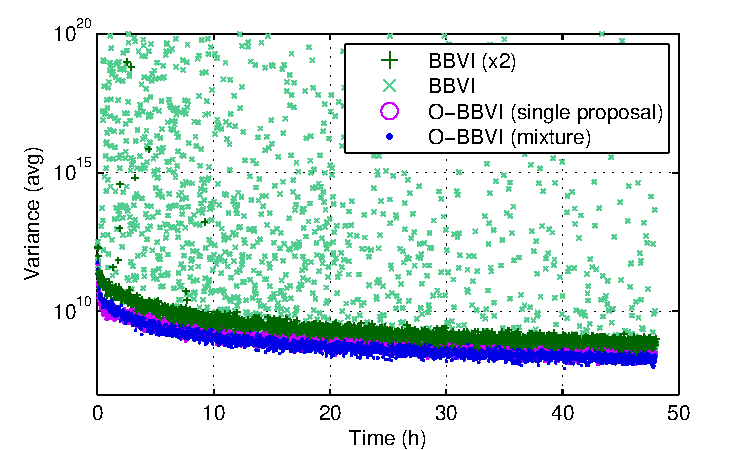
\includegraphics[width=0.85\columnwidth]{plots/gamNormTS_varall_vs_t.pdf}}\\ \vspace*{-7pt}
  \subfloat[Traceplot of the \gls{ELBO}.\label{fig:gamNormTS_elbo_vs_t}]{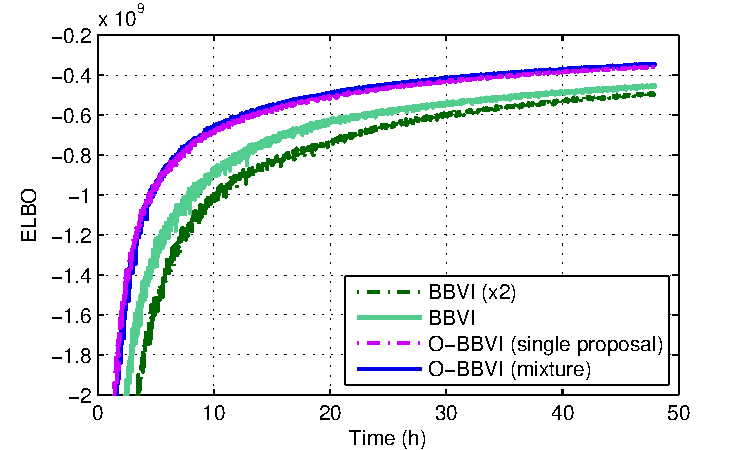
\includegraphics[width=0.85\columnwidth]{plots/gamNormTS_elbo_vs_t.pdf}}\\ \vspace*{-12pt}
  \subfloat[Predictive performance (higher is better).\label{fig:gamNormTS_err_vs_t}]{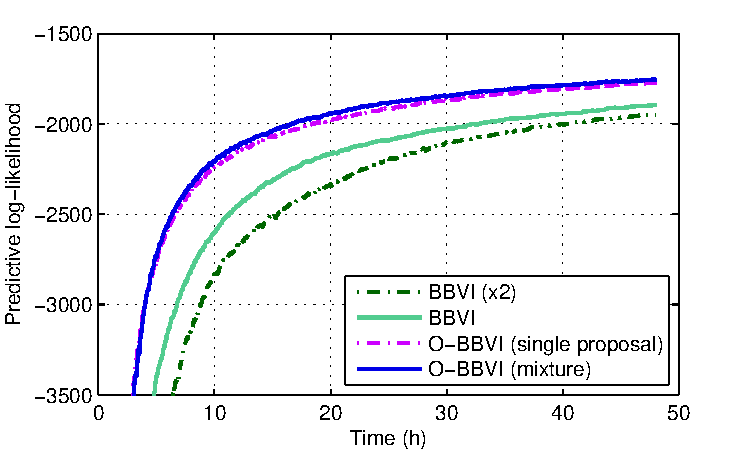
\includegraphics[width=0.85\columnwidth]{plots/gamNormTS_err_vs_t.pdf}}\\ \vspace*{-4pt}
  \caption{Results for the \gls{GNTS} model. Both versions of \acrshort{OBBVI} converge faster than \gls{BBVI}.\label{fig:gamNormTS}} \vspace*{-8pt}
\end{figure}

\begin{figure}[t]
  \centering
  \subfloat[Averaged sample variance of the estimator.\label{fig:poissonDEF_varall_vs_t}]{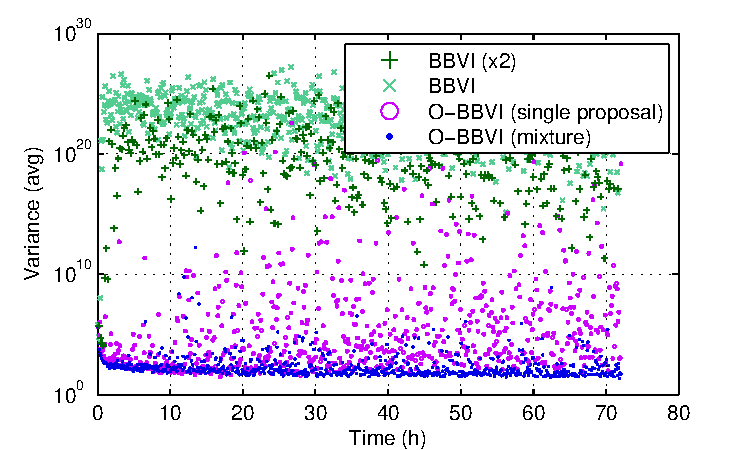
\includegraphics[width=0.85\columnwidth]{plots/poissonDEF_varall_vs_t.pdf}}\\ \vspace*{-7pt}
  \subfloat[Traceplot of the \gls{ELBO}.\label{fig:poissonDEF_elbo_vs_t}]{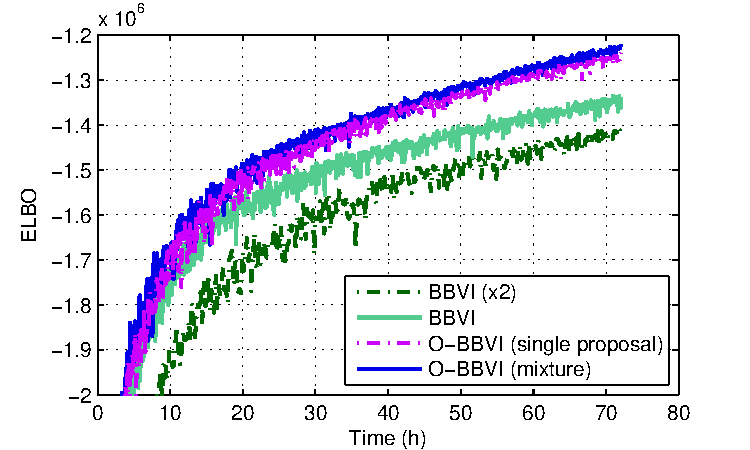
\includegraphics[width=0.85\columnwidth]{plots/poissonDEF_elbo_vs_t.pdf}}\\ \vspace*{-12pt}
  \subfloat[Predictive performance (lower is better).\label{fig:poissonDEF_err_vs_t}]{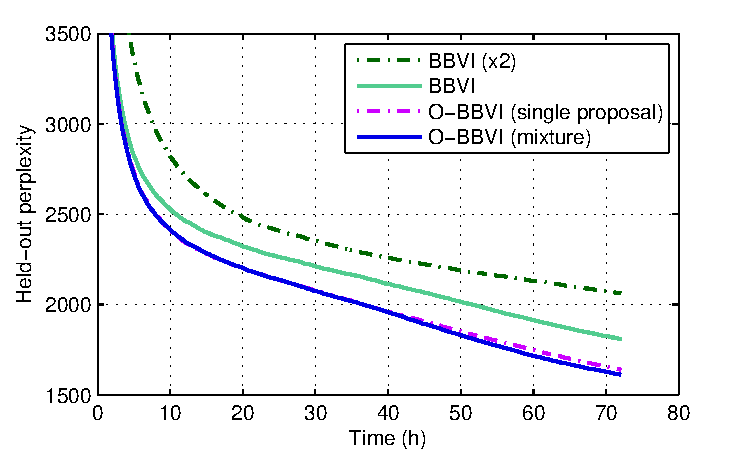
\includegraphics[width=0.85\columnwidth]{plots/poissonDEF_err_vs_t.pdf}}\\ \vspace*{-4pt}
  \caption{Results for the Poisson \gls{DEF} model. Both versions of \acrshort{OBBVI} converge faster than \gls{BBVI}.\label{fig:poissonDEF}} \vspace*{-8pt}
\end{figure}

%we do not compare with local expectation gradients because they are not available for the Poisson nor the gamma distributions. Instead,

%For local expectation gradients (labeled as ``Legrad'' in the plots), since they use numerical quadratures or a weighted summation to estimate the expectations, there is no need to estimate the control variates, and therefore the estimation of the gradient requires $8$ function evaluations only.

%%% Local Variables:
%%% mode: latex
%%% TeX-master: "obbvi-uai"
%%% End:
